\documentclass[11pt,letterpaper,openany]{report}
\usepackage{amsmath}
\usepackage{amssymb}
\usepackage{bm}
\usepackage{graphicx}
\usepackage{alltt}
\usepackage{url}

   \setlength{\hoffset}{-1in}
   \setlength{\voffset}{-1in}
   \setlength{\oddsidemargin}{1.00in}
   \setlength{\textwidth}{6.5in}
   \setlength{\topmargin}{0.50in}
   \setlength{\headheight}{0.25in}
   \setlength{\headsep}{0.25in}
   \setlength{\textheight}{9.0in}

%>>>>>>>>>>>>>>>>>>>>>>>>>>>>>>>>>>>>>>>>>>>>>>>>>>>>>>>>>>>>>>>>>>>>>>>>>>>>>>
\begin{document}
%>>>>>>>>>>>>>>>>>>>>>>>>>>>>>>>>>>>>>>>>>>>>>>>>>>>>>>>>>>>>>>>>>>>>>>>>>>>>>>


%%%%%%%%%%%%%%%%%%%%%%%%%%%%%%%%%%%%%%%%%%%%%%%%%%%%%%%%%%%%%%%%%%%%%%%%%%%%%%%
%   Title Page                                                                %
%%%%%%%%%%%%%%%%%%%%%%%%%%%%%%%%%%%%%%%%%%%%%%%%%%%%%%%%%%%%%%%%%%%%%%%%%%%%%%%
\title{Hamer Collision Model User Manual V.1.0}
\author{prepared by Lars Holmstrom for Hamer Environmental, L.P.}
\date{}
\maketitle

%%%%%%%%%%%%%%%%%%%%%%%%%%%%%%%%%%%%%%%%%%%%%%%%%%%%%%%%%%%%%%%%%%%%%%%%%%%%%%%
%   Table of Contents                                                         %
%%%%%%%%%%%%%%%%%%%%%%%%%%%%%%%%%%%%%%%%%%%%%%%%%%%%%%%%%%%%%%%%%%%%%%%%%%%%%%%
\tableofcontents

%%%%%%%%%%%%%%%%%%%%%%%%%%%%%%%%%%%%%%%%%%%%%%%%%%%%%%%%%%%%%%%%%%%%%%%%%%%%%%%
%   Main Document                                                             %
%%%%%%%%%%%%%%%%%%%%%%%%%%%%%%%%%%%%%%%%%%%%%%%%%%%%%%%%%%%%%%%%%%%%%%%%%%%%%%%
\chapter{Getting Up and Running}
\section{Installation}
\subsection{Program Files}
The model software package includes three files required for installation:
\begin{itemize}
  \item \textbf{MCRInstaller.exe}: This is the Matlab Runtime Component required to run the model. It will only need to be installed once on each machine.
  \item \textbf{AvianCollisionModel.ctf}: This file is an archive of files that are part of the model application. It will be expanded into the appropriate directory structure the first time the model is run.
  \item \textbf{AvianCollisionModel.exe}: This is the actual model application. This is what is launched to run the model.
\end{itemize}

\subsection{Installing the Matlab Runtine}
The Matlab Runtime installs all of the components necessary to run applications developed using the Matlab computing
environment. To install it, simply launch the \textbf{MCRInstaller.exe} application and follow the prompts.

\subsection{Installing the Avian Collision Model}
To install the model, two steps must be followed:
\begin{enumerate}
  \item Create a directory to run the model from. It is suggested that \newline
  \verb"c:/Program Files/AvianCollisionModel" \newline
  be used to make future upgrades easier.
  \item Copy both \textbf{AvianCollisionModel.ctf} and \textbf{AvianCollisionModel.exe} into this directory.
\end{enumerate}

\section{Updating}
When updates to the model become available, two steps must be followed to update the model installation:
\begin{enumerate}
  \item Delete the contents of the model installation directory for created above.
  \item Copy the new versions of \textbf{AvianCollisionModel.ctf} and \textbf{AvianCollisionModel.exe} into the
empty directory
\end{enumerate}

\section{Launching the Application}
To start the model application, double click on the \textbf{AvianCollisionModel.exe} file.

\section{Saving and Loading Model Configurations}
Using the \textbf{File} menu, the current model configuration can be saved to a file for later retrieval. Use the
\textbf{Open} option in the \textbf{File} menu to load a saved configuration.

\chapter{Running the Avian Collision Model}
\section{Bird Characteristics}
The avian collision model allows for the specification of the following bird specific parameters:
\begin{itemize}
  \item Wingspan
  \item Length
  \item Mean speed
  \item Mean direction
  \item Mean flightpath height
  \item Variance of the flightpath height
\end{itemize}
The wingspan and length are species dependent, while the other parameters are determined from field survey data. The
speed and direction parameters both assume a uni-modal distribution. This is clearly not true when the birds are, for
example, coming inland in the evening and are seabound at dawn, resulting in a bi-modal distribution. In this case,
different estimates should be produced for each mode. Flightpath height further assumes that the distribution in
normally distributed (gaussian) in order to model the distribution of height using the variance statistic alone. The
flightpath distribution in the horizontal axis is assumed to be uniformly distributed, meaning that flightpaths in the
horizontal plane are all equally likely.

\section{Wind Characteristics}
The avian collision model allows for the specification of the following wind specific parameters:
\begin{itemize}
  \item Mean speed
  \item Mean direction
\end{itemize}
The wind speed and direction are used in conjunction with the bird speed and direction to calculate both the
orientation of the turbines relative to the flightpath and the orientation of the bird relative to the turbine as it
passes through the turbine plane. Again, the distribution of these two parameters are assumed to be uni-modal. If this
is not a reasonable assumption, then multiple runs of the model may need to be performed or the model updated to
account for different statistical distributions.

If the \textbf{Enable} checkbox is disabled, than it is assumed that no wind data is available for the site. It is
further assumed that the bird is flying downwind.

\section{Survey Characteristics}
The avian collision model allows for the specification of the following survey specific parameters:
\begin{itemize}
  \item Horizontal radar range
  \item Passage rate
\end{itemize}
The horizontal radar range is required to determine the proportion of the measured passage rate that will pass through
the wind farm. If, for example, the recorded passage rate is 10 birds per day, but the horizontal span of the wind farm
perpendicular to the flightpath is half of the horizontal radar range, than the effective passage rate will be 5 birds
per day.

\section{Turbine Characteristics}
The avian collision model allows for the specification of the following turbine specific parameters:
\begin{itemize}
  \item Number of rotors
  \item Radius of the turbine
  \item Radius of the nacelle
  \item Angular velocity
  \item Maximum rotor chord length
\end{itemize}
%PUT THIS BACK IN
%These characteristics are typically all available from the turbine manufacturer. Since the formulas describing the
%exact shape of the turbine blade is often proprietary, a general formula was adapted from \cite{Tucker1996} which is
%based off of the maximum rotor length of blade. This specification is often available from the manufacturer.

To make it easy to switch between common turbine types, there is a drop down menu which allows a selection from the
following varieties:
\begin{itemize}
  \item GE 1.5se
  \item Gamesa 80
  \item Vestas V80
  \item Vestas V90
\end{itemize}
After selecting any of these items, any of the turbine parameters can still be individually customized.

If the \textbf{Enable} checkbox is disabled, than the turbine is not included in the avian collision estimate. This is
useful for estimating the collision rate due to the tower components alone.

\section{Tower Characteristics}
The avian collision model allows for the specification of the following tower specific parameters:
\begin{itemize}
  \item Height
  \item Diameter at base
  \item Diameter at hub
  \item Largest diameter
  \item Height at largest diameter
\end{itemize}
The tower is assumed to be circular. Other tower configurations would require an update to the model. This may be
useful, for example, in estimating collision rates with cell towers or other static structures (when the turbine
component is disabled as described above).

\section{Wind Farm Characteristics}
The avian collision model allows for the specification of the following wind farm specific parameters:
\begin{itemize}
  \item Number of rows
  \item Number of column
  \item Distance between rows
  \item Distance between columns
\end{itemize}
The wind farm layout is assumed to be in a grid formation. Other configurations will require an update to the model.

\section{Model Selection}
The avian collision model allows for the selection of the turbine collision model to use:
\begin{itemize}
  \item Hamer
  \item Tucker
  \item Podolski
\end{itemize}
The Hamer model can account for cases where the bird is traveling neither upwind or downwind, resulting in a rotated
turbine relative to the flight path. The Tucker model is the accepted standard in the field but assumes downwind or
upwind flight paths. The Hamer and Tucker models provide nearly identical results when this assumption holds. The
Podolski model uses a different analytical approach for calculating the turbine collision probabilities which, in my
opinion, are not as rigorous or sound as the Hamer or Tucker models.

\section{Show Single Turbine Probabilities}
When this checkbox is checked, only the turbine collision probability calculation is performed, and none of the wind
farm calculations. This can speed up the process when comparing the 3 model types for a set of model inputs.

\chapter{Model Output}
Currently, the model produces a number of figures in addition to the final collision rate estimate. These figures are
helpful both in interpreting and validating the results. Furthermore, they may be used for inclusion in reports making
use of the model. Following is a description of each figure type along with the calculation(s) it represents.

\section{Turbine Collision}
Figure \ref{fig.Turbine} displays the result of the individual turbine collision calculations. The color scale at each
point indicates the probability of collision with a bird flying in a straight path whose nose intersects the plane of
the rotating turbine at that point. A value of 0 indicates no chance of collision (for example, all of the areas
outside the radius of the turbine), and a value of 1 indicates a 100\% chance of collision (for example, the center of
the turbine where the stationary nacelle is). The figure shows the turbine from the perspective of the bird, so it may
be rotated, resulting in an oval rather than a circle.

The mean collision probability displayed in the figure title indicates the mean collision probability across the
surface of the turbine as seen by the bird. The mean rotation adjusted collision probability indicates the mean
collision probability across the surface of the turbine, accounting for any rotation of the turbine (this is the value
used in the collision rate estimates). For downwind flight (dead-on), these two values are identical. As the rotation
of the turbine increases, so does the mean collision probability across its surface, since the bird will spend more
time in the turbine rotor plane. Since the profile of the turbine is reduced, however the rotation adjusted collision
rate does not necessarily increase.

\section{Wind Farm Layout}
Figure \ref{fig.WindFarm} shows the layout of the specified wind farm against a generic background image. It indicates
both the spatial dimensions, as well as the relative rotor size and orientation.

\section{Compass and Directions}
Figure \ref{fig.Directions} displays the relevant directions included in the collision estimate: the bird flight path,
the wind direction, and the bird's orientation. When the wind direction is non-zero and different than the flight path
direction, the bird will have an orientation that is rotated from its actual flight path. For example, if the bird is
pointed north, but there is a wind blowing to the west, the flight path with be north-west.

\section{Wind Farm Collision Probabilities}
Figure \ref{fig.WindFarmProbs} shows the wind farm, from the perspective of the bird, and the associated collision
probabilities for each possible flight path. As with figure \ref{fig.Turbine}, the scale is from 0 (no probability of
collision) to 1 (definite collision). Note that the towers and nacelles are static and both result in 100\% collision
probabilities.

\section{Flight Path Probability Densities}
Figure \ref{fig.FlightPathProbs} indicates the probability density of where the bird's flight path will likely be based
on the mean and variance of the flight path heights specified in the model inputs. This probability density answers the
question "assuming a bird is flying through the the survey area, what flight path is it likely to take?". All flight
paths in the horizontal direction are equally likely (by model design), but are distributed about the mean height in
the vertical direction. In this figure, the mean flight path height is equal to the highest point of the turbine
rotation, so only 50\% of the probability density is represented, indicating that only 50\% of the flight paths would
fall below this height and may result in a collision.

\section{Combined Wind Farm / Flight Path Collision Probabilities}
As discussed above, figure \ref{fig.FlightPathProbs} indicates the probable flight paths of a bird passing through the
survey area while figure \ref{fig.WindFarmProbs} indicates the probability of a collision with the wind farm for each
possible flight path. By multiplying these two arrays together, flight path by flight path, we generate figure
\ref{fig.Final}.

By summing (integrating) over the entire array, we can estimate the probability of a collision for a single bird
passing through the wind farm area. After accounting for the proportion of the survey site occupied by the wind farm
area, the avoidance rate of each bird, and the computed passage rate of the survey site, we generate the final
estimated collision rate for the wind farm.

\begin{figure}
   \centering
   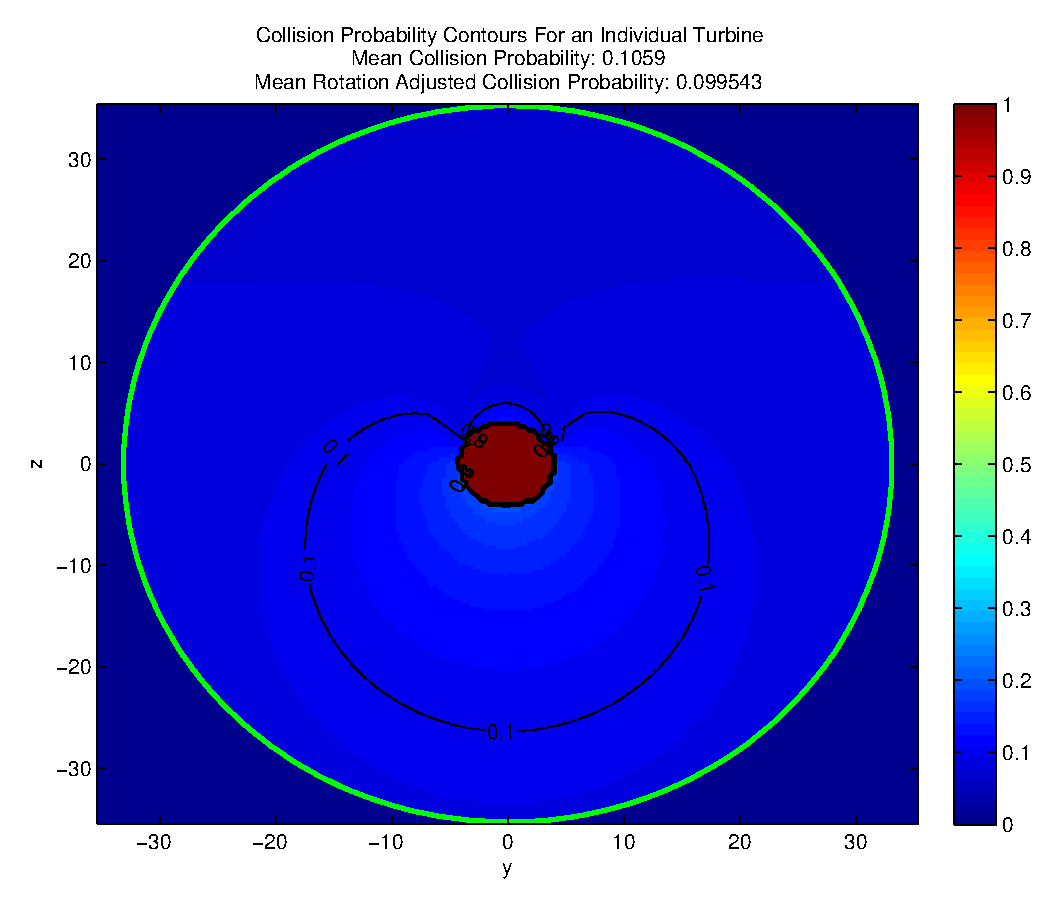
\includegraphics[width=0.75\columnwidth]{Turbine}
   \caption{}
   \label{fig.Turbine}
\end{figure}

\begin{figure}
   \centering
   \includegraphics[width=0.75\columnwidth]{WindFarm}
   \caption{}
   \label{fig.WindFarm}
\end{figure}

\begin{figure}
   \centering
   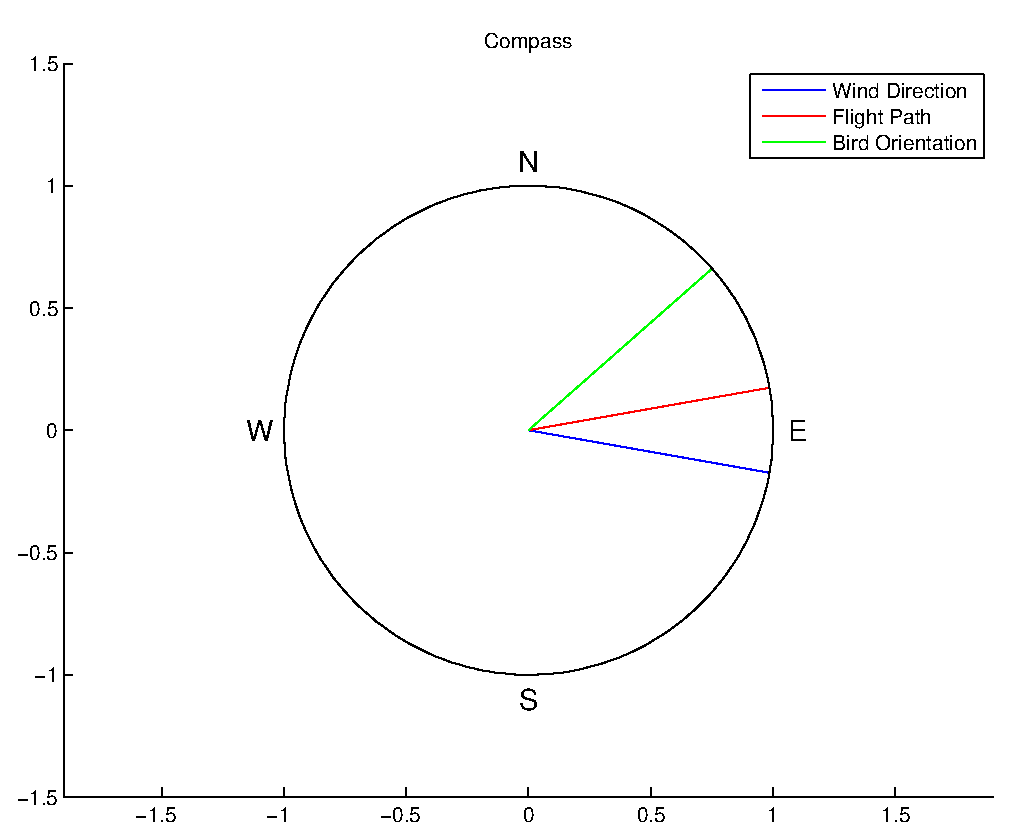
\includegraphics[width=0.5\columnwidth]{Directions}
   \caption{}
   \label{fig.Directions}
\end{figure}

\begin{figure}
   \centering
   \includegraphics[width=1\columnwidth]{WindFarmProbs}
   \caption{}
   \label{fig.WindFarmProbs}
\end{figure}

\begin{figure}
   \centering
   \includegraphics[width=1\columnwidth]{FlightPathProbs}
   \caption{}
   \label{fig.FlightPathProbs}
\end{figure}

\begin{figure}
   \centering
   \includegraphics[width=1\columnwidth]{Final}
   \label{fig.Final}
   \caption{}
\end{figure}

%\bibliography{IEEEAbrv,references}
%\bibiliography{IEEEAbrv,"C:/Documents and Settings/lars/Desktop/references"}
%\bibliographystyle{IEEETran}

%>>>>>>>>>>>>>>>>>>>>>>>>>>>>>>>>>>>>>>>>>>>>>>>>>>>>>>>>>>>>>>>>>>>>>>>>>>>>>>
\end{document}
%>>>>>>>>>>>>>>>>>>>>>>>>>>>>>>>>>>>>>>>>>>>>>>>>>>>>>>>>>>>>>>>>>>>>>>>>>>>>>>
